
\documentclass{article}
\usepackage[utf8]{inputenc}
\usepackage{graphicx}

\begin{document}
\title{Day 2}

\author{\emph{Teemu Sarapisto}}
\maketitle

\newcommand{\aaa}[3]{%
  \fbox{\includegraphics[height=30mm]{#1}} \quad
  \fbox{\includegraphics[height=30mm]{#2}} \quad
  \fbox{\includegraphics[height=30mm]{#3}} \par}
\newcommand{\bbb}[3]{%
  \medskip\noindent\aaa{#1}{#1-#2}{#1-#3}}

\newpage

\setlength{\fboxsep}{0pt}%

\section{Hands-on day 2}
Hola world

\subsection{Use OpenCV’s morphological dilation and closing with different structuring element shapes and sizes to fill in the “holes” in the strawberries. Try to also clean away the noisy stray pixels with mild erosion or opening}
    \begin{figure}[h]
        \centering
        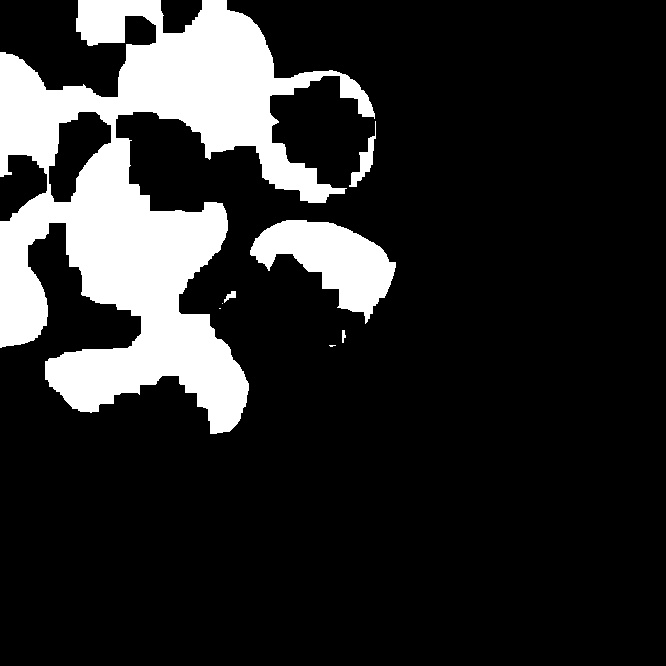
\includegraphics[scale=0.50]{morph}
    \end{figure}

\subsection{What seems to be the best operations, structuring element shapes and their sizes? In which order were they performed?}

\begin{itemize}
    \item Closing operation with a rectangular kernel
    \item Dilation operation with a rectangular kernel
    \item Closing operation 2 with a rectangular kernel
    \item Erosion operation with a rectangular kernel
\end{itemize}

\subsection{Apply a series of OpenCV’s Gaussian blurring operations with increasing kernel sizes to get smoothed versions of the image}
Kernel sizes: 3/5 11/15 27/27 37/47

\fbox{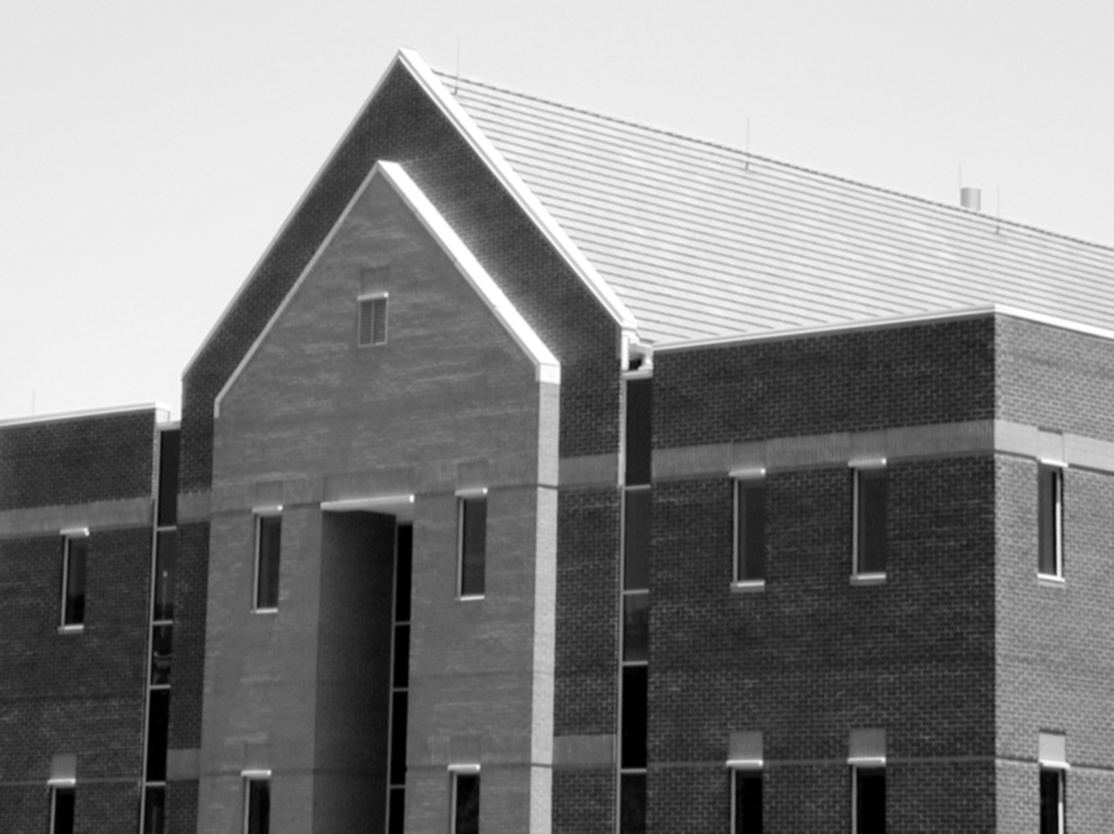
\includegraphics[scale=0.2]{gaussed3-5}} \quad
\fbox{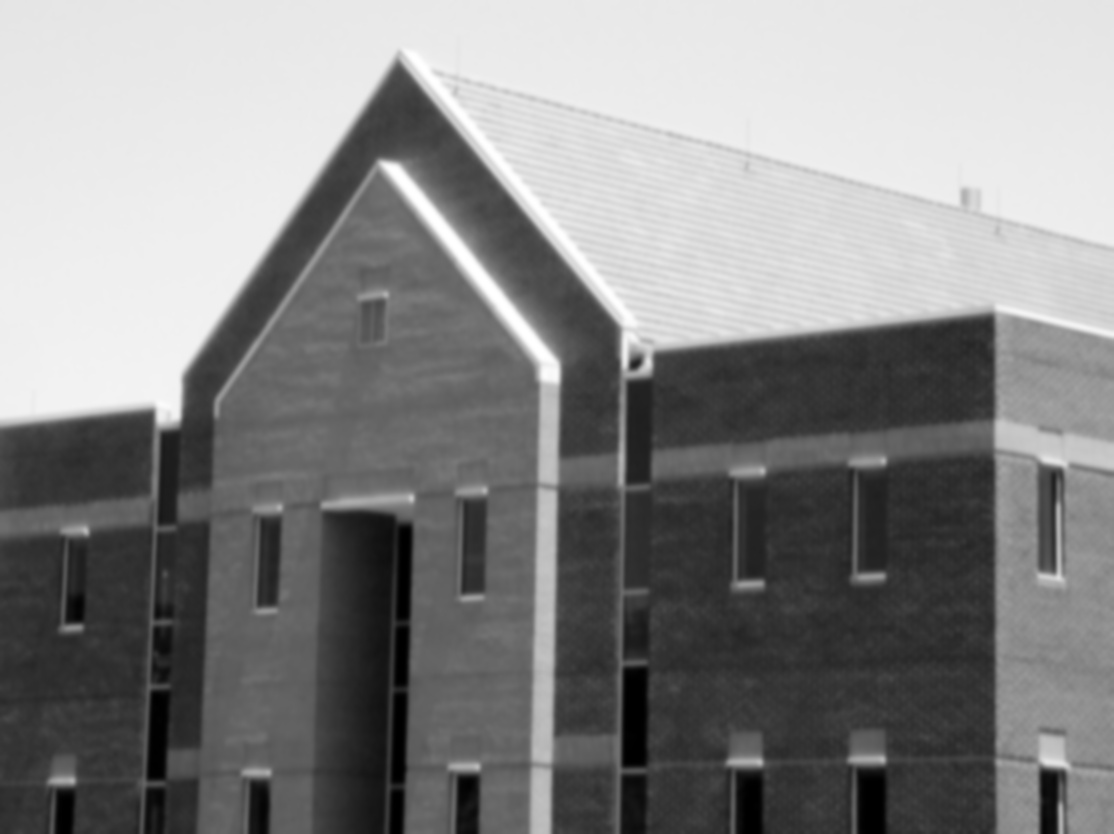
\includegraphics[scale=0.2]{gaussed11-15}} \quad
\fbox{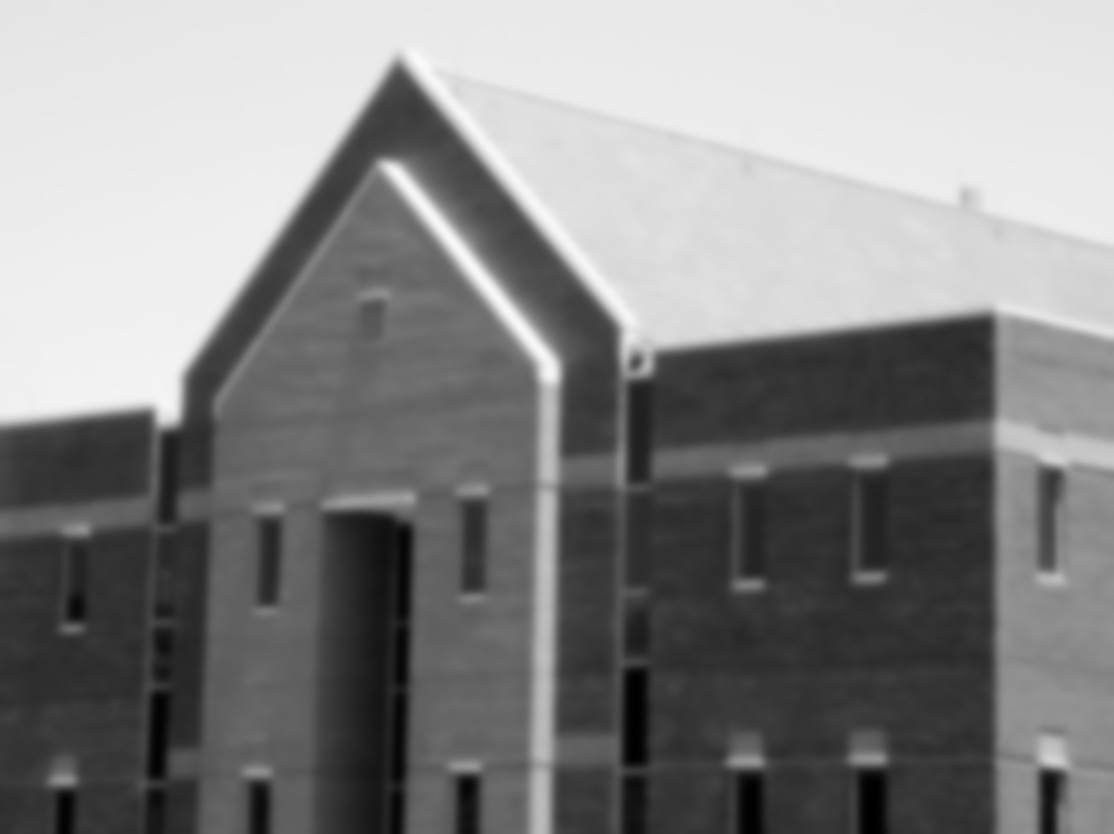
\includegraphics[scale=0.2]{gaussed27-27}} \quad
\fbox{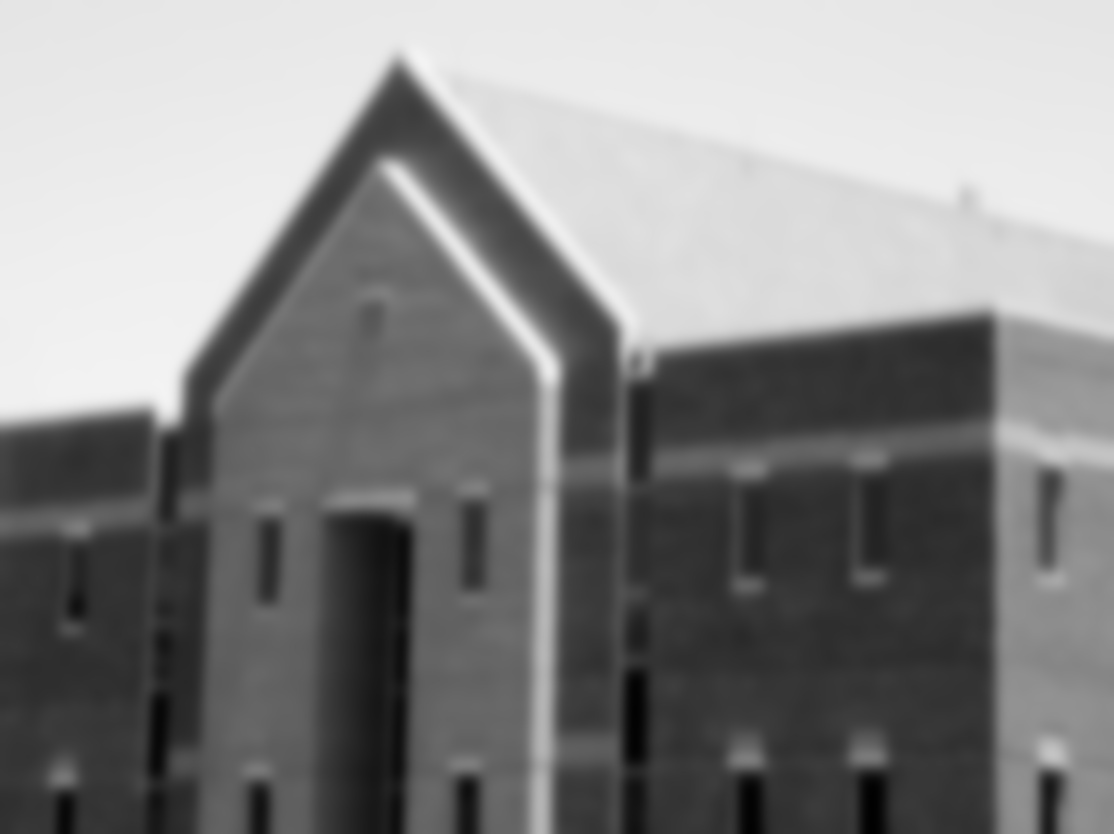
\includegraphics[scale=0.2]{gaussed37-47}} \par

\subsection{Apply OpenCV’s Laplace filtering to the blurred images}
oispa kaljaa

\fbox{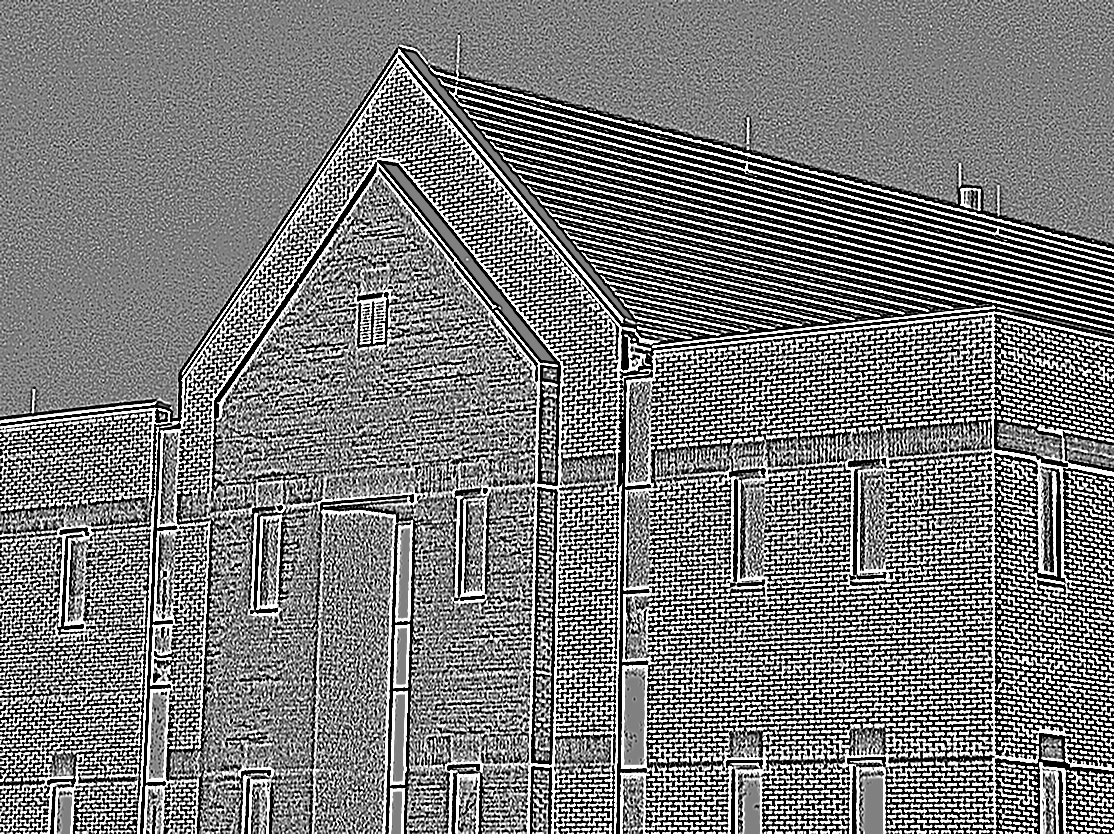
\includegraphics[scale=0.2]{laplace1}} \quad
\fbox{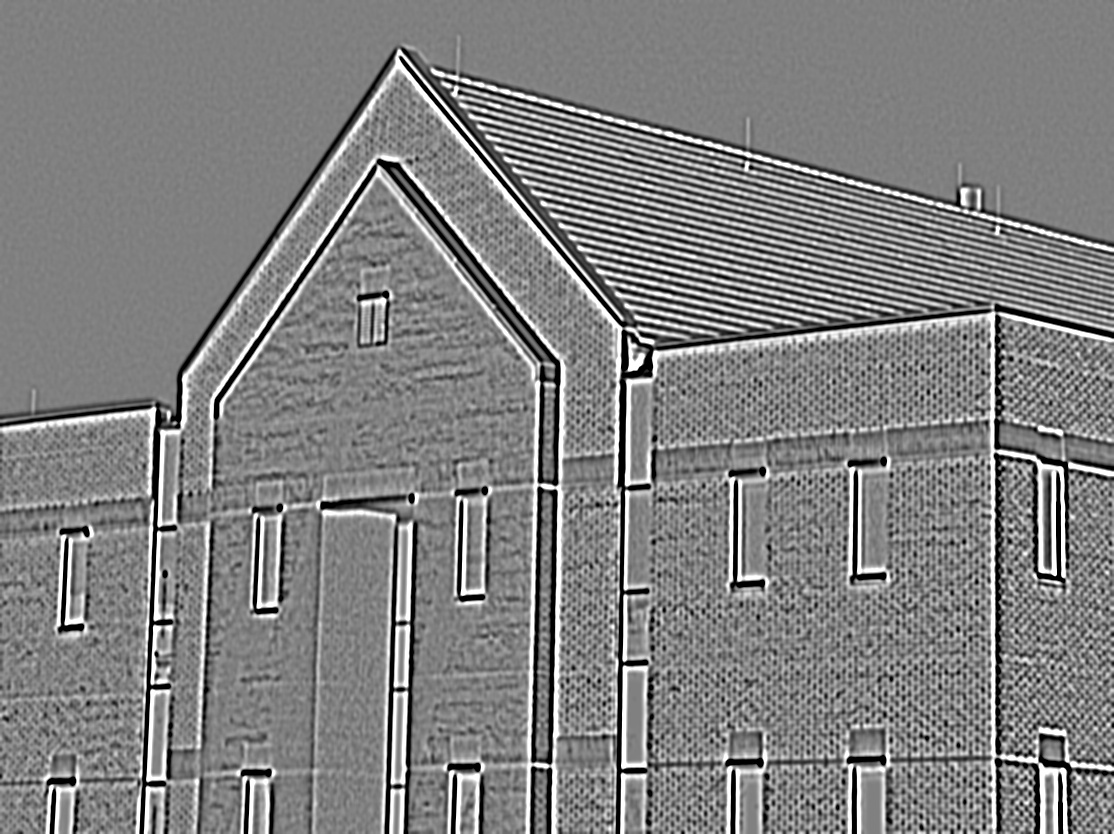
\includegraphics[scale=0.2]{laplace2}} \quad
\fbox{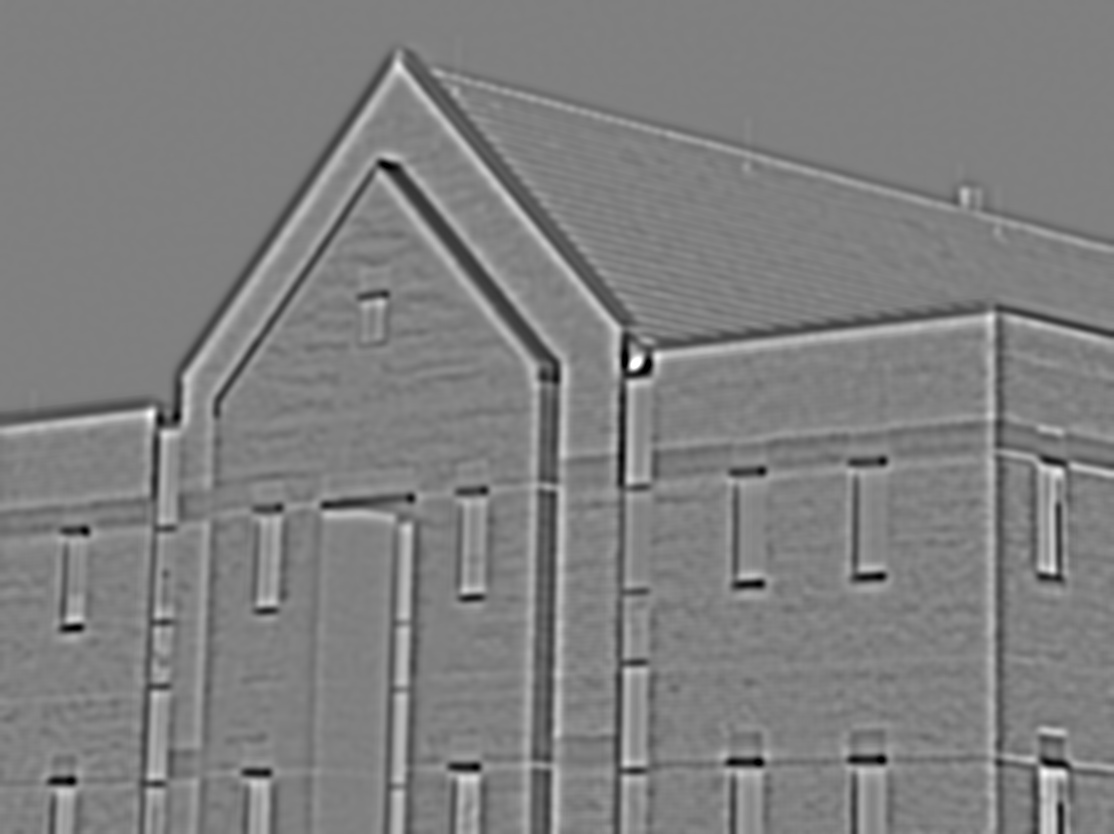
\includegraphics[scale=0.2]{laplace3}} \quad
\fbox{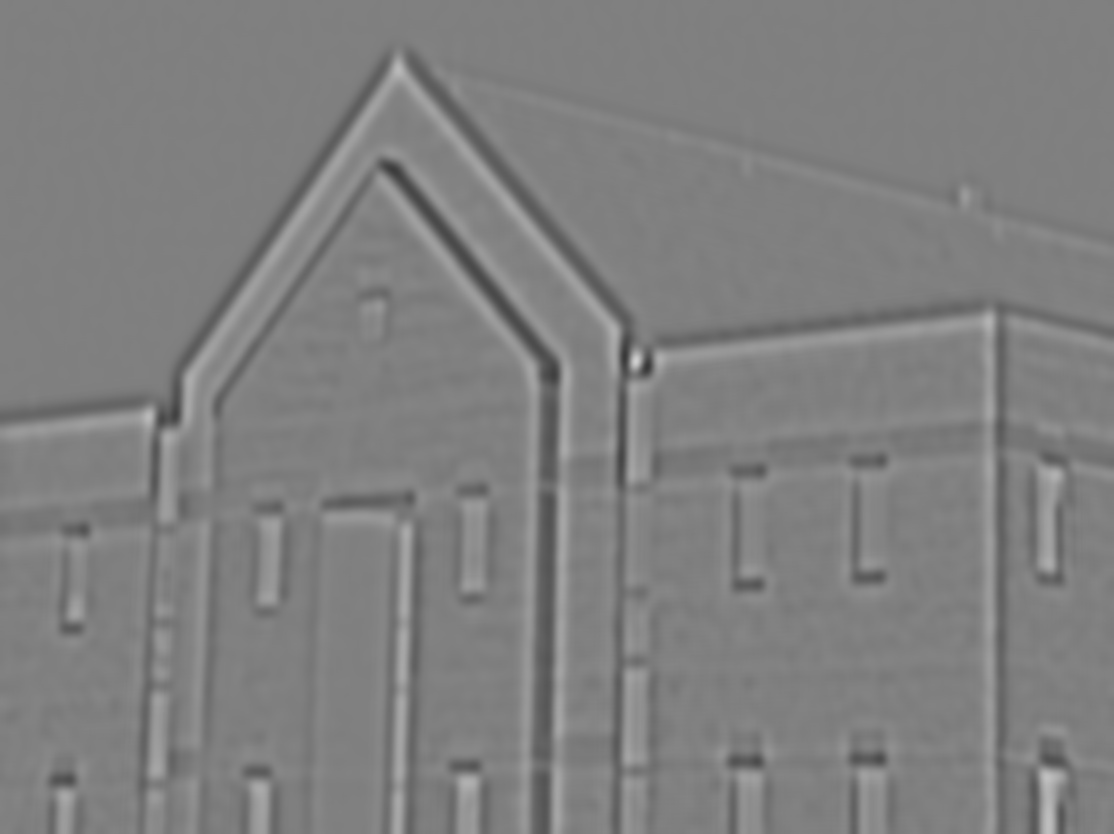
\includegraphics[scale=0.2]{laplace4}} \par

\subsection{Analyze how the size of the detected details increases with the increasing blur size}
\fbox{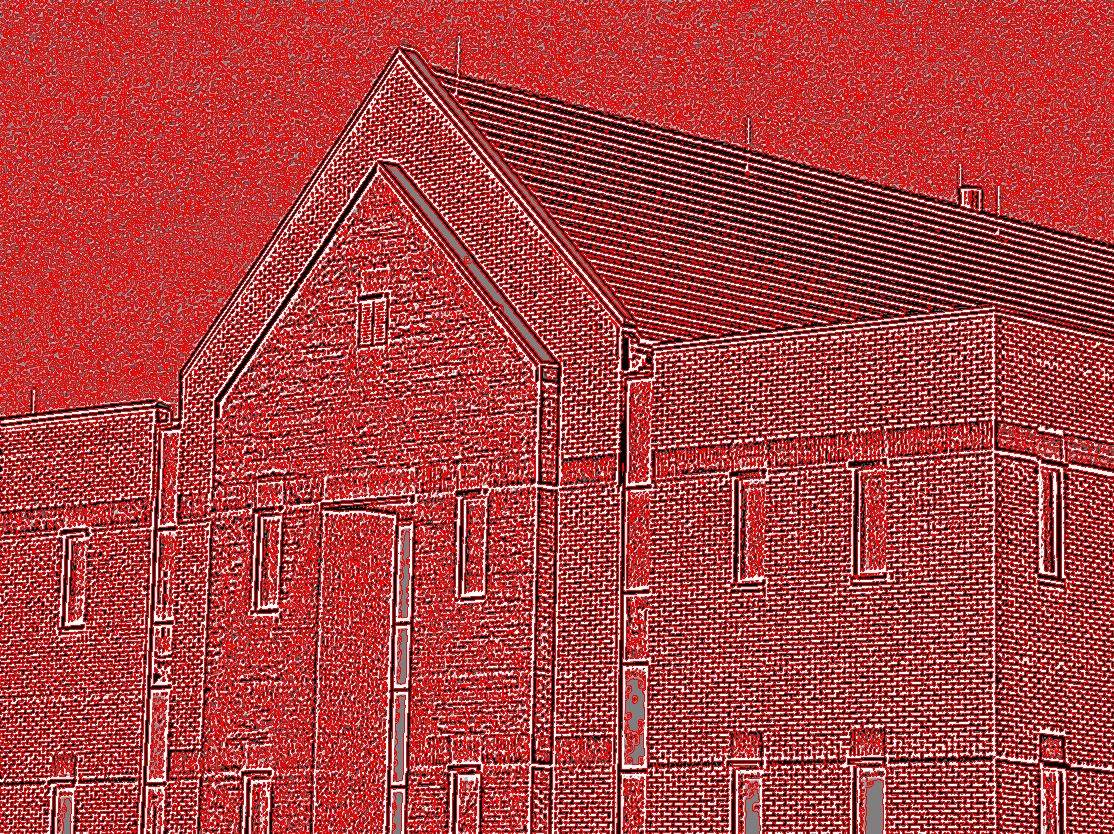
\includegraphics[scale=0.2]{laplace1_zcross}} \quad
\fbox{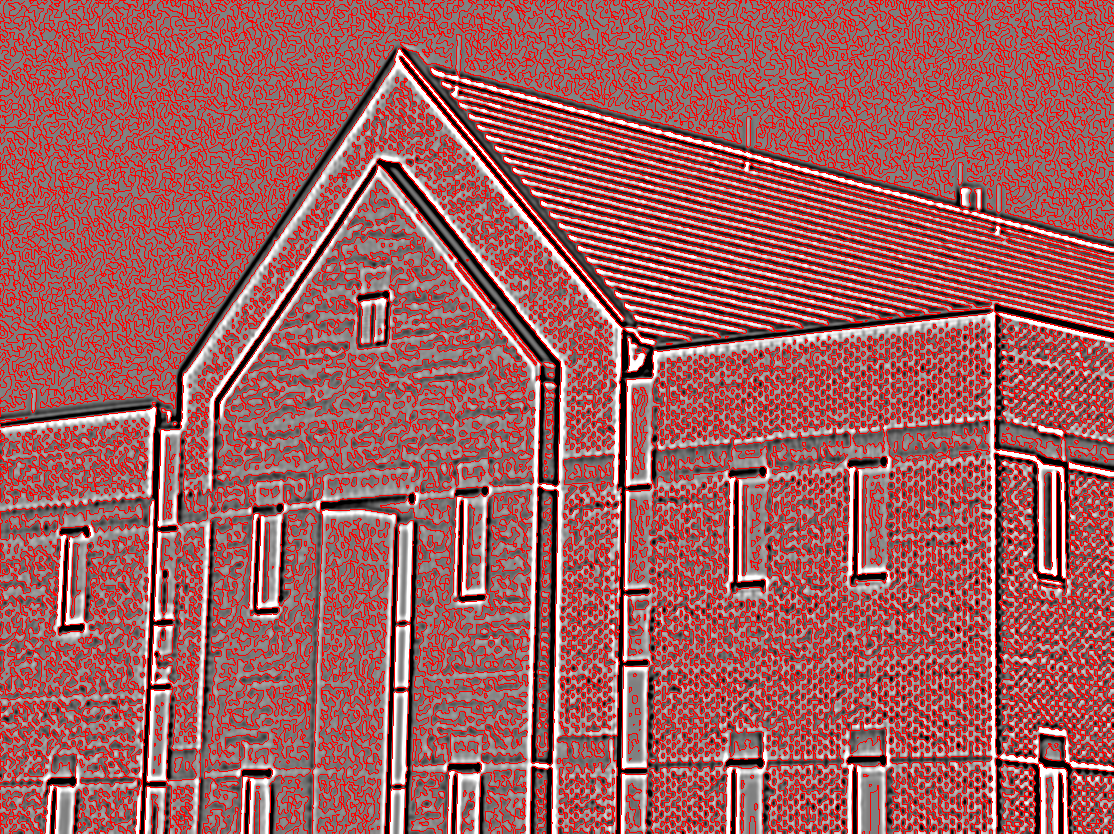
\includegraphics[scale=0.2]{laplace2_zcross}} \quad
\fbox{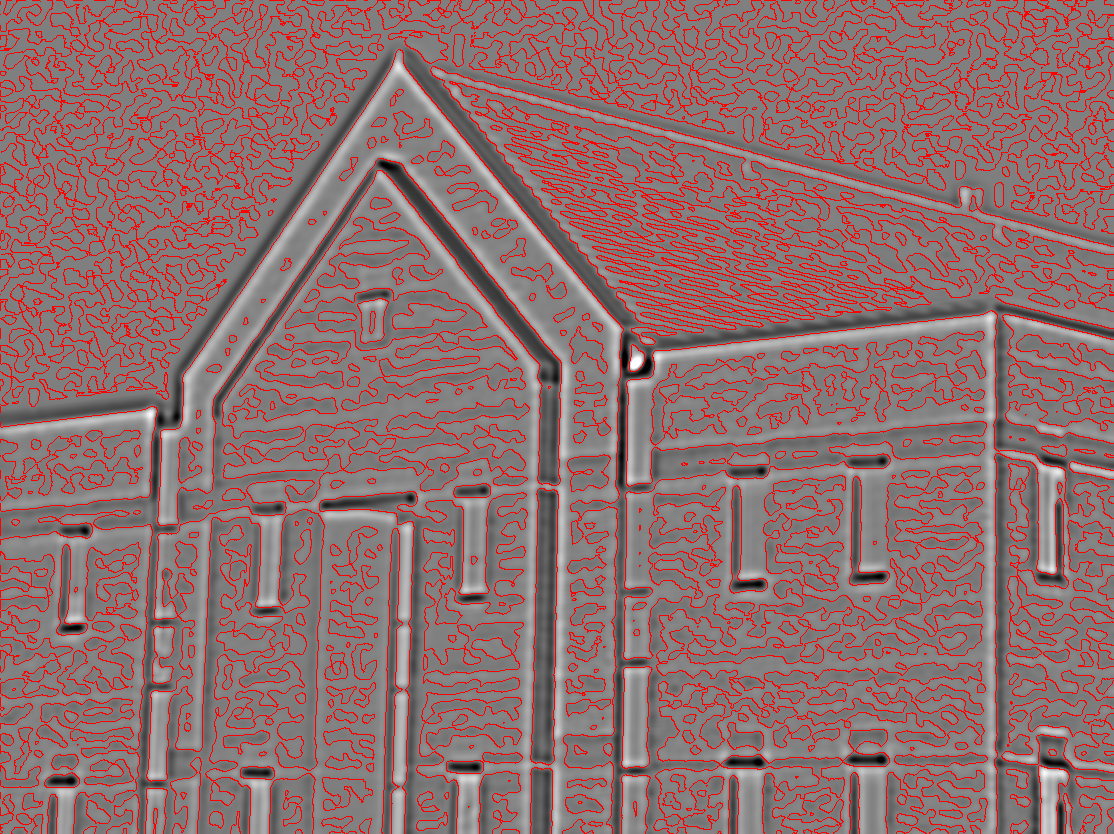
\includegraphics[scale=0.2]{laplace3_zcross}} \quad
\fbox{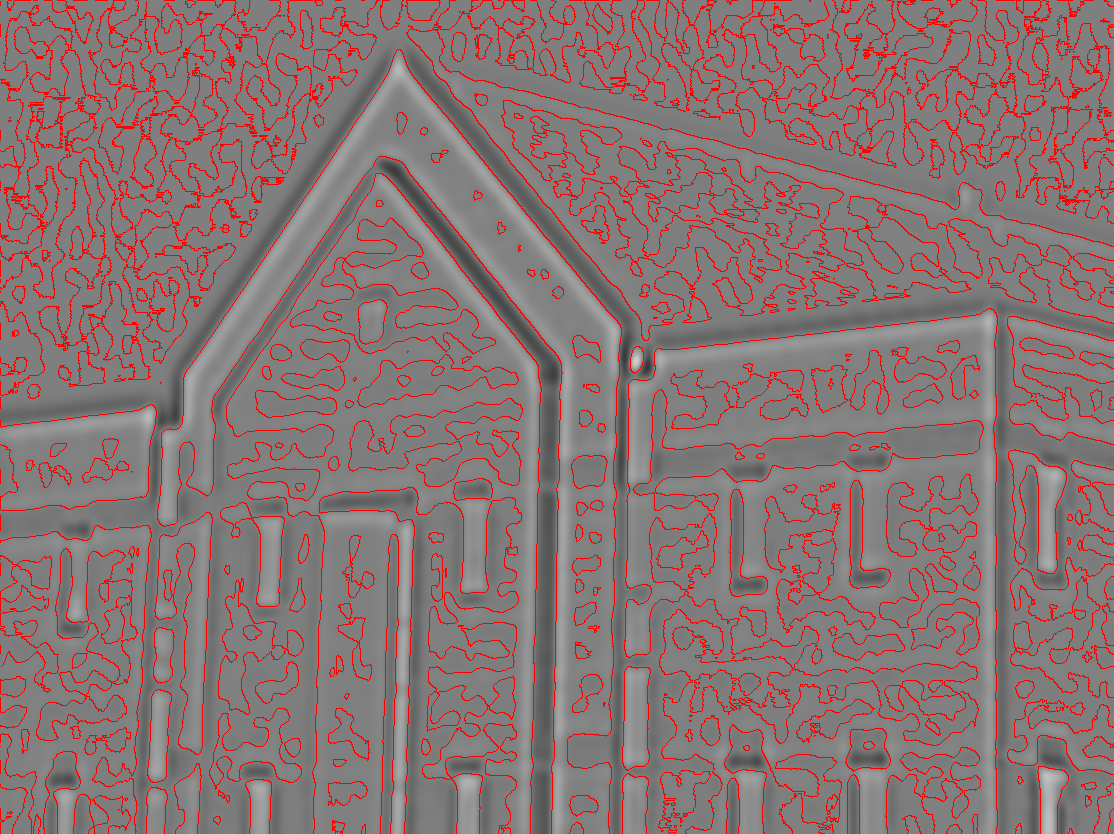
\includegraphics[scale=0.2]{laplace4_zcross}} \par
With the increasing blur size the size of the detected details increases.:

\subsection{how long it took}
Around 4 hours

\begin{verbatim}
  import cv2
  import numpy as np
  import matplotlib.pyplot as plt
  import matplotlib.cm as cm
  from scipy import ndimage as nd
  from scipy.spatial import distance


  # We will use the image, strawberries-binary.pbm that is a binary mask or segmentation result showing the red strawberry pixels of the previous home work

  strawberries_red = cv2.imread('strawberries-binary.pbm')

  #Read the image in and scale it to have “white” values 1 for the strawberry pixels and “black” values 0 for background pixels
  binary_strawberries = strawberries_red / 255

  #Use OpenCV’s morphological dilation and closing with different structuring element shapes and sizes to fill in the “holes” in the strawberries
  #Try to also clean away the noisy stray pixels with mild erosion or opening
  rect_kernel = cv2.getStructuringElement(cv2.MORPH_RECT,(5,5))
  elliptical_kernel = cv2.getStructuringElement(cv2.MORPH_ELLIPSE,(5,5))
  cross_kernel = cv2.getStructuringElement(cv2.MORPH_CROSS,(5,5))

  closing = cv2.morphologyEx(binary_strawberries, cv2.MORPH_CLOSE, rect_kernel)

  dilation = cv2.dilate(closing, rect_kernel, iterations = 2)

  closing2 = cv2.morphologyEx(dilation, cv2.MORPH_CLOSE, rect_kernel)

  kernel = np.ones((5,5),np.uint8)
  erosion = cv2.erode(closing2, kernel, iterations = 3)

  #cv2.imshow("homma", erosion * 255)
  cv2.imwrite("morph.jpg", erosion * 255)
  #cv2.waitKey()


  ###Next we use building.tiff to study scale space filtering, Laplacian of Gaussian filtering and edge detection by zero crossings
  # Ookoo kuulostaapa hyveltä

  ###Read the image in and scale it as a single-channel (greyscale) image in range [0,1]
  building = cv2.imread('building.tiff', cv2.IMREAD_GRAYSCALE) / 255

  ###Apply a series of OpenCV’s Gaussian blurring operations with increasing kernel sizes to get smoothed versions of the image

  #cv2.GaussianBlur(src, ksize, sigmaX[, dst[, sigmaY[, borderType]]])  dst
  gaussed1 = cv2.GaussianBlur(building, (3,5), 0)
  gaussed2 = cv2.GaussianBlur(building, (11,15), 0)
  gaussed3 = cv2.GaussianBlur(building, (27,27), 0)
  gaussed4 = cv2.GaussianBlur(building, (37,47), 0)

  cv2.imwrite('gaussed3-5.jpg', gaussed1 * 255)
  cv2.imwrite('gaussed11-15.jpg', gaussed2 * 255)
  cv2.imwrite('gaussed27-27.jpg', gaussed3 * 255)
  cv2.imwrite('gaussed37-47.jpg', gaussed4 * 255)

  #Apply OpenCV’s Laplace filtering to the blurred images
  #When saving the Laplace images for the report, multiply them with a proper constant, add 0.5 and clip to [0,1] to improve their informativeness
  def clip(i):
      return np.clip(i, 0, 1)

  kernel_size = 3
  scale = 1
  delta = 0
  laplace1 = cv2.Laplacian(gaussed1, cv2.CV_64F)
  laplace2 = cv2.Laplacian(gaussed2, cv2.CV_64F)
  laplace3 = cv2.Laplacian(gaussed3, cv2.CV_64F)
  laplace4 = cv2.Laplacian(gaussed4, cv2.CV_64F)

  cv2.imwrite('laplace1.jpg', clip(laplace1 * 40 + 0.5) * 255)
  cv2.imwrite('laplace2.jpg', clip(laplace2 * 40 + 0.5) * 255)
  cv2.imwrite('laplace3.jpg', clip(laplace3 * 40 + 0.5) * 255)
  cv2.imwrite('laplace4.jpg', clip(laplace4 * 40 + 0.5) * 255)

  #Write your own function to detect zero crossings (aka sign changes) in the Laplace filtered images
  ###Compare each pixel value’s sign (-1, 0 or +1) to that of the neighboring pixel on the left and above: If all signs are equal, the pixel is not a zero crossing pixel, otherwise it is

  def zero_cross(A):
      new = np.zeros(A.shape)
      for x in range(A.shape[1]):
          for y in range(A.shape[0]):

              if x == 0 and y == 0: 
                  new[y][x] = 0
              elif x == 0:
                  if np.sign(A[y][x]) != np.sign(A[y][x-1]):
                      new[y][x] = 1
                  else:
                      new[y][x] = 0 
              elif y == 0:
                  if np.sign(A[y][x]) != np.sign(A[y-1][x]):
                      new[y][x] = 1
                  else:
                      new[y][x] = 0 
              else:
                  if np.sign(A[y][x]) != np.sign(A[y-1][x]) or np.sign(A[y][x]) != np.sign(A[y][x-1]):
                      new[y][x] = 1
                  else:
                      new[y][x] = 0
      return new


  zbuilding = zero_cross(building)
  #print(zbuilding[23])

  #cv2.imwrite('zero_building.jpg', zbuilding)

  #Mark the zero crossing pixels with red color in the images
  def color_zero(zero_cross, original):
      original_uint8 = np.array(original, dtype=np.uint8)
      new = cv2.cvtColor(original_uint8,cv2.COLOR_GRAY2BGR)
      for x in range(zero_cross.shape[0]):
          for y in range(zero_cross.shape[1]):
              if zero_cross[x,y] == 1:
                  new[x,y] = [0,0,255]
              else:
                  new[x,y] = original[x,y]
      
      return new

  #cv2.imshow('haloo', color_zero(zbuilding, building))
  #cv2.waitKey()
      

  #Analyze how the size of the detected details increases with the increasing blur size
  laplace1_cross = zero_cross(laplace1)
  laplace2_cross = zero_cross(laplace2)
  laplace3_cross = zero_cross(laplace3)
  laplace4_cross = zero_cross(laplace4)
  cv2.imwrite('laplace1_zcross.png', color_zero(laplace1_cross, clip(laplace1 * 40 + 0.5) * 255))
  cv2.imwrite('laplace2_zcross.png', color_zero(laplace2_cross, clip(laplace2 * 40 + 0.5) * 255))
  cv2.imwrite('laplace3_zcross.png', color_zero(laplace3_cross, clip(laplace3 * 40 + 0.5) * 255))
  cv2.imwrite('laplace4_zcross.png', color_zero(laplace4_cross, clip(laplace4 * 40 + 0.5) * 255))
  #cv2.waitKey()
  #Report again how long it take to complete these assignments
\end{verbatim}

\section{Homework}

\end{document}
%  LocalWords:  Jorma Laaksonen pdf py tex OpenCV libopencv dev jpg
%  LocalWords:  highgui imgproc imgcodecs greyscale png opencv ing
%  LocalWords:  texlive includegraphics Exactum Gür Ersalan
